\documentclass[]{beamer}
%%%%%%%%%%%%%Bibliography
\usepackage[backend=bibtex, url=false,
bibstyle=ieee,firstinits=true]{biblatex}
\renewcommand*{\thefootnote}{} %No symbol or marker
\renewcommand{\footnotesize}{\scriptsize}
%%%%%%%%%%%%%%%%%


\usepackage{xcolor}
\definecolor{chamois}{RGB}{255,255,240}
\definecolor{darkbrown}{RGB}{124,79,0}
\definecolor{UniBlue}{RGB}{83,101,130}

\definecolor{hellgelb}{rgb}{1,1,0.8}
\definecolor{colKeys}{rgb}{0,0,1}
\definecolor{colIdentifier}{rgb}{0,0,0}
\definecolor{colComments}{rgb}{1,0,0}
\definecolor{colString}{rgb}{0,0.5,0}

\usefonttheme{professionalfonts}
\usepackage{tgadventor}
\renewcommand*\familydefault{\sfdefault}
\usepackage[T1]{fontenc}
\usepackage{microtype}


\newcommand{\topline}{%
  \tikz[remember picture,overlay] {%
    \draw[brown,ultra thick] ([yshift=-1.8cm]current page.north west)-- ([yshift=-1.8cm,xshift=\paperwidth]current page.north west);} }

\renewcommand{\topline}{}

\setbeamertemplate{frametitle}{\begin{minipage}[b][1.8cm][c]{\textwidth}%
	\centering%
	\insertframetitle\\\insertframesubtitle
	\end{minipage}}
	

\addtobeamertemplate{frametitle}{}{\topline%
}

\setbeamertemplate{navigation symbols}{}
\setbeamercolor{background canvas}{bg=chamois}
\setbeamercolor{itemize item}{fg=brown}
%\setbeamertemplate{itemize item}{\maltese}
\setbeamercolor{itemize subitem}{fg=brown}
%\setbeamertemplate{itemize subitem}{\begin{rotate}{90}$\diamondsuit$\end{rotate}}

\setbeamercolor{title}{fg=UniBlue}
\setbeamercolor{frametitle}{fg=UniBlue}    
\setbeamerfont{frametitle}{size=\Large}

\setbeamercolor{author}{fg=darkbrown}
\setbeamercolor{institute}{fg=darkbrown}
\setbeamercolor{date}{fg=darkbrown}


\setbeamercolor{structure}{fg=UniBlue}
\setbeamercolor{alerted text}{fg=UniBlue}
\setbeamercolor{alerted text}{fg=UniBlue}
\setbeamercolor{normal text}{fg=darkbrown!50!black}
\setbeamercolor{math text}{fg=darkbrown}
\setbeamercolor{math text displayed}{fg=darkbrown}



\addtobeamertemplate{block begin}{%
	\setlength{\textwidth}{0.8\textwidth}%
}{}
\setbeamercolor{block title}{bg=darkbrown!40,fg=darkbrown!90}
\setbeamercolor{block body}{bg=darkbrown!20,fg=UniBlue}
\setbeamercolor{block title alerted}{bg=yellow!60,fg=red}
\setbeamercolor{block body alerted}{bg=hellgelb!80,fg=UniBlue}

\AtBeginSection[]{
	\begin{frame}
		\vfill
		\centering
		\begin{beamercolorbox}[sep=8pt,center,shadow=true,rounded=true]{title}
			\usebeamerfont{title}\insertsectionhead\par%
		\end{beamercolorbox}
		\vfill
	\end{frame}
}

\usepackage{standalone}
\usepackage{graphicx}
\graphicspath{{../figs/}}
\usepackage{pifont}% http://ctan.org/pkg/pifont
\usepackage{amsthm}
\usepackage{amsmath}
\usepackage{amssymb}
\usepackage{mathtools}
\usepackage{multirow}
\usepackage{resizegather}

\usepackage{rotating}
%\usepackage{fontspec}
\usepackage{microtype}
                        
                               

%%%%%%%%%%%%%%%%%%%%%%%%%%
% PGFPLOTS
\usepackage{pgfplots}
\pgfplotsset{compat=1.12}
\usepackage{booktabs, array} % Generates table from .csv
\usepackage{pgfplotstable}

\newcolumntype{C}[1]{>{\centering\arraybackslash}m{#1}}

\pgfplotstableset{percent style/.style=}
		}},
		%
		every head row/.style={after row=\midrule},
	}

%%%%%%%%%%%%%%%%%%%


\usepackage{arrayjobx}
\usepackage{xifthen}
\usepackage{tikz,textcomp}
\usetikzlibrary{positioning}
\newcommand{\fullpagetikz}[1]{{\input{#1}}}
\newcommand{\widthtikz}[2]{\resizebox{#1\textwidth}{!}{
		\centering
		\input{#2}}}
\newcommand{\fullwidthtikz}[1]{\resizebox{0.9\textwidth}{!}{
		\centering
		\input{#1}}}



%%%%%%%%%%%%%%%%%%%%%%%%%%%%%%%%%%%%%%%%%%%%%%%%%%%%%%%%%%%%%%%%%%%%%%%%%%%%%%%%%%%%%%%%%%
\renewcommand{\c}{\tilde{c}}
\newcommand{\st}{\tilde{s}}
\newcommand{\x}{\tilde{x}}
\renewcommand{\t}{\tilde{t}}
\newcommand{\N}{\mathbb{N}}
\newcommand{\R}{\mathbb{R}}
\newcommand{\V}{\mathcal{V}}
\newcommand{\B}{\mathcal{B}}
\newcommand{\s}{w_{\blacktriangleright}}
\renewcommand{\ss}{w_{\triangleright}}
\newcommand{\e}{w_{\triangleleft}}
\newcommand{\ee}{w_{\blacktriangleleft}}
\newcommand{\W}{\mathcal{W}}

\newcommand{\displayunskip}{\vspace{0pt}}

\bibliography{master}


\author{\textbf{Lyndon White},\\ Roberto Togneri, Wei Liu, Mohammed Bennamoun}
\institute{School of EE\&C Engineering\\The University of Western Australia}
\title{Generating Sentences from the Sum of their Contents}
\subtitle{A greedy algorithms for sentence generation from sum of word embeddings representations}

\begin{document}
\frame{\maketitle}

\begin{frame}[label=task]{We have turned sentences into numeric vectors, now we want to turn them back.}

	\begin{enumerate}
		\item<1-> It was the best of times, it was the worst of times
		\item<1->  $[−0.79, 1.27, 0.28, ..., −1.29]$
		\item<1-> It was the worse of times, it was the best of times
	\end{enumerate}
\end{frame}

\begin{frame}{The use of an ideal generation system is in allowing manipulation in the vector domain}
	\small Input Sentences \hfill Manipulate Numbers \hfill Output Sentences
	\vspace{0.5cm}
	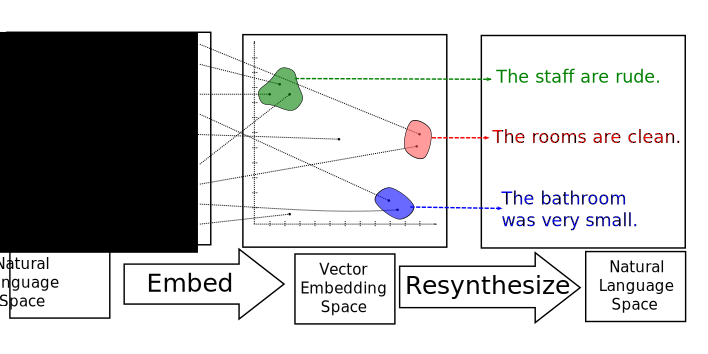
\includegraphics[scale=0.5]{workflow}
\end{frame}

\begin{frame}{Related problems}
	\begin{block}{Related problems include}
	\begin{itemize}
		\item Sequence Memorisation
		\item Sequence-Sequence Learning
	\end{itemize}
	\end{block}
	\begin{block}{}
		\begin{itemize}
			\item Sentence generation is different from either.
			\item Going from a vector representation that only encodes \alert{meaning}
			\item Rather than from one that encodes \alert{memory} of meaning.
		\end{itemize}
	\end{block}

\end{frame}

\againframe{task}


\begin{frame}{Related work: Dependancy Tree RAE}
	\begin{block}<1->{Method}
		\begin{itemize}
			\item Input as tree structured of word embeddings combined with single layer nets
			\item Output same structure
			\item Use Back Propagating Through Structure in training
		\end{itemize}
	\end{block}
	\begin{block}<2->{}
		\begin{itemize}
			\item Produces fairly clean paraphrases 
			\item Requires output tree structure to be provided
		\end{itemize}
	\end{block}
	\footfullcite{iyyer2014generating}
\end{frame}



\begin{frame}{Related work: LSTM + Variational Autoencoder}
	\begin{block}<1->{Method}
			\begin{itemize}
				\item LSTM encoding step
				\item Variational Autoencoder Representation step
				\item LSTM decoding step
			\end{itemize}
	\end{block}
	\begin{block}<2->{}
		\begin{itemize}
			\item Smooth ``deformation'' between sentences
			\item Several other uses beyond just generation
			\item No demonstration on sentences with more than 6 words
		\end{itemize}
	\end{block}
	\footfullcite{Bowman2015SmoothGeneration}
\end{frame}

\againframe{task}

\begin{frame}<1-3>[label=twostep]{We broke the problem down into two subproblems.}
	\vfill

	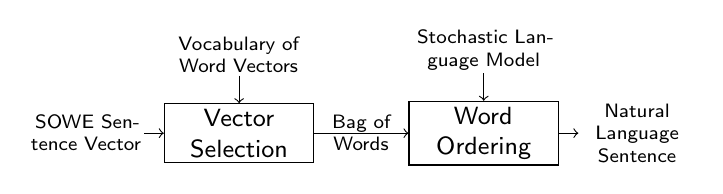
\begin{tikzpicture}[
		every node/.style={ text width=5em,
			align=center,
			font=\scriptsize\sffamily,
			inner sep=1pt
		},
		proc/.style= {draw,
			font=\small\sffamily,
			inner sep = 2pt
		}
		]
		\onslide<1,3->{
			\node (input) [inner sep=-4pt] {SOWE Sentence Vector};
			\node (selection) [proc, right = 0.7em of input]{Vector\\ Selection};
			\node (vocab) [above = 1em of selection]{Vocabulary of Word Vectors};
			\draw[->] (input) -- (selection);
			\draw[->] (vocab) -- (selection);
		}
		\onslide<2->{
			\node (ordering) [proc, right = 3.4em of selection]{Word\\ Ordering};
		}

		
		\draw[->] (selection) -- (ordering) node[midway] {Bag of\\Words};
		\onslide<2,3->{
			\node (output) [inner sep=-4pt, right=0.7em of ordering] {Natural Language Sentence};
			\node (lm) [above = 1em of ordering] {Stochastic Language Model};
			\draw[->] (lm) -- (ordering);
			\draw[->] (ordering) -- (output);
			
		}
	\end{tikzpicture}
	\vfill
	\only<1,4>{\alert{Vector Selection}: Select which word vectors go into the sum}
	
	\only<2,4>{\alert{Word Ordering}: Find them most likely order of words}
	
	\only<3>{They are however both \alert{NP-Hard}
		%\\But both are similar to well studied problems
		}
	\vfill
\end{frame}

\newcommand{\vectorselectionproblemdefn}{Find the \alert{inclusion vector} $\c=[c_1,c_2,...c_n]\in\N_0^n$ to \alert{minimise}
	 $\displaystyle d(\st,\:\: \sum_{\x_j\in\V}\:\x_{j}\,c_{j})$ 
}

\begin{frame}{We get a bag of words by minimising an objective function}
	\vectorselectionproblemdefn
	\vfill
	\begin{description}
		%\item<1->[Target Output] It was the best of times, it was the worst of times
		\item<2->[Input Vector]  $\st=[−0.79, 1.27, 0.28, ..., −1.29]$
		\vfill
		\item<3->[Vector Selection] $\displaystyle
			\begin{aligned}%
			f(\c)&=\quad1\times[−0.19, 0.50, 0.14, ..., −0.59]\\
			&\quad+2\times[-0.15, 0.19, 0.03, ..., -0.17]\\
			&\quad+\qquad...\\
			&\quad+0\times[−0.19, 2.10, 1.34, ..., 1.20]\\
			&\quad+1\times[−0.79, 1.27, 0.28, ..., −1.29]
		\end{aligned}
		$
		\vfill
		\item<4->[BOW] \texttt{\{best: 1,times: 2, worst: 1, \\it: 2, of: 2, the: 2, was: 2,, : 1\}}
	\end{description}
\end{frame}

\begin{frame}{How to solve objective function? Greedily}
	\vectorselectionproblemdefn
		\vfill
	\begin{itemize}
		\item<1-> Similarities to \alert{Knapsack} family of problems.
		\item<2-> Very high dimensionality of selection vector\begin{itemize}
			\item $n$ is given by vocabulary size ($n=|\V|$)
			\item $\approx170,000$ for Books Corpus
			\end{itemize}
		\item<3-> A Greedy Algorithm is linear time in $n$ 
	\end{itemize}
	\vfill
\end{frame}


\begin{frame}{Run until convergence}
	\vspace{-1em}
	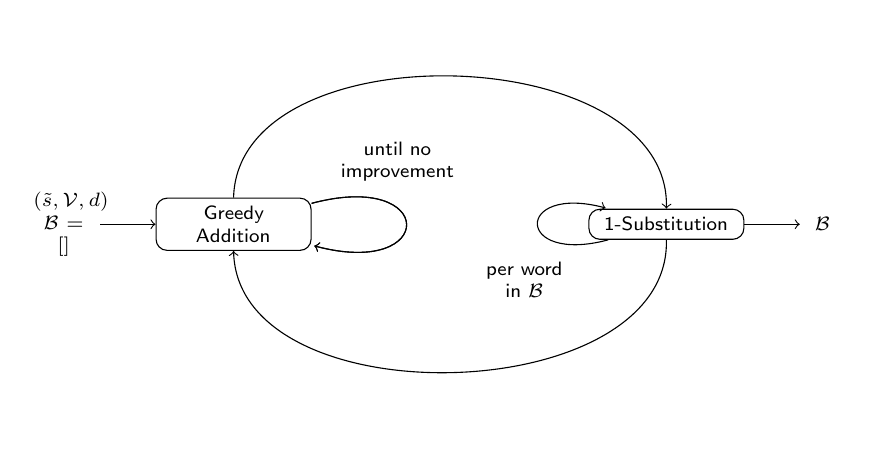
\begin{tikzpicture}[
		every node/.style={ text width=5em,
			align=center,
			font=\scriptsize\sffamily,
			inner sep=3pt,
		},
		]

		\node (input) [text width=2em] {$(\st,\V,d)$\\$\B=[]$};
		\node (addition) [draw, rounded corners, right = 2em of input]{Greedy Addition};
		\node (substitution) [draw, rounded corners, right = 10em of addition]{1-Substitution};
		\node (output) [right = 2em of substitution,text width=1em] {$\B$};
		\draw[->] (input) -- (addition);
		\path[->] (addition) edge[loop right] (addition);
		\node [above right=0.4em of addition, text width = 5em] {\scriptsize  until no \\ improvement};
		\path[->] (substitution) edge[loop left] (substitution);
		\path[->] (addition) edge[loop right] (addition);
		\node [below left=0.7em of substitution, text width = 3em] {\scriptsize  per word \\ in $\B$};
		\path[->] (addition) edge [bend left=90,looseness=1] (substitution);
		\path[->] (substitution) edge [bend left=90,looseness=1] (addition);
		\draw[->] (substitution) -- (output);
			
	\end{tikzpicture}
	
	%\begin{block}
		\begin{itemize}
			\item \alert{Greedy Addition}: add word to bag that gets us closest
			\item \alert{1-Substitution}: Reconsider past choices
		\end{itemize}
	%\end{block}
		
		\footfullcite{White2015BOWgen}
	
		
\end{frame}



\againframe<4>{twostep}

\begin{frame}{Now that we have a bag of words, we need to order them to get a sentence.}
	\vfill
		Find the most-likely ordering, of the bag of words.
	\vfill
	\begin{description}
		\item<1->[Input Vector]  $[−0.79, 1.27, 0.28, ..., −1.29]$
		\item<1->[Bag of Words]  \texttt{\{best: 1,times: 2, worst: 1,\\ it: 2, of: 2, the: 2, was: 2,, : 1\}}
		\vspace{1em}
		\item<1->[Output Sentence] It was the worse of times, it was the best of times
	\end{description}
	\vfill
\end{frame}

\begin{frame}{A language model tells us the probability of a word sequence.}
	\begin{itemize}
		\item based on corpus statistics
		\item Trigram language model: $P(W_3=buns\:|\:W_1=hot, W_2=crossed)$
		\item With the the Markov Assumption, that the transition probability only depends on the current state.
		\pause
		\item Bayesian Chain Rule: probability of sequence \\$P([w_1,w_2,w_3,w_4,w_5])=$
		$$\qquad \quad P(w_1,w_2)\cdot P(w_3|w_1,w_2)\cdot P(w_4|w_2,w_3) \cdot P(w_5|w_3,w_2)$$
		
	\end{itemize}
	
\end{frame}


\begin{frame}{We can formulate word ordering as a Mixed Integer Programming (MIP) problem}
	\begin{itemize}
		\item There exist very fast MIP solvers.
		\item This gave multiple orders of magnitude improvement over Best First Search.
		\item and even over incomplete Beamer Search.
	\end{itemize}
\end{frame}

\begin{frame}{Word Sequencing as a Travelling Salesman Problem}
	\vspace{-1em}
	\fullwidthtikz{../figs/ordergraphpaper}
	\footfullcite{Horvat2014}
	 
\end{frame}

\begin{frame}{Edge Constraints}
	\vspace{-1em} 
	\fullwidthtikz{../figs/ordergraphpaper}
	
	\alert{Markov Consistency:} $(w_aw_b)\to (w_cw_d) \iff w_b==w_c$
	\displayunskip
	\begin{gather*}
	\tau[\langle w_{i},w_{j}\rangle,\,\langle w_{j},w_{k}\rangle] = %\\
	\begin{cases}
	\multirow{2}{*}{1} & \mathrm{if\,transition\,from} \\
	& \langle w_{i},w_{j}\rangle \to \langle w_{j},w_{k}\rangle
	\;\mathrm{ occurs} \\
	0  & \mathrm{otherwise}
	\end{cases}
	\end{gather*}
\end{frame}


\begin{frame}{Word sequencing graph objective}
	\vspace{-1em}
	\fullwidthtikz{../figs/ordergraphpaper}
	
	\alert{Edge cost:} $C[\langle w_{i},w_{j}\rangle,\langle w_{j},w_{k}\rangle]=-\log\left(P(w_{k}|w_{i},w_{j})\right)$
	\displayunskip
	\begin{gather*}
	C_{total}(\tau)= \sum_{\forall w_i,w_j,w_k \in \W^{3}}
		\;\tau[\langle w_{i},w_{j}\rangle,\,\langle w_{j},w_{k}\rangle] \cdot C[\langle w_{i},w_{j}\rangle,\,\langle w_{j},w_{k}\rangle]
	\end{gather*}

\end{frame}


\begin{frame}{Word Use Constraint}
	\vspace{-1em}
	\fullwidthtikz{../figs/ordergraphpaper}
	
	\alert{Districts:} Every word must be used exactly once
	$\forall w_{i}\in\W\backslash\{\s,\ee\}$:
	\displayunskip
	\begin{gather*}
	\sum_{\forall\langle w_{i},w_{j}\rangle\in S(w_{i}\rangle} \:
	\sum_{\forall\langle w_{h},w_{i}\rangle\in\W^{2}}
	\tau[\langle w_{h},w_{i}\rangle,\,\langle w_{i},w_{j}\rangle]=1
	\end{gather*}
\end{frame}



\begin{frame}{Single Path Constraint}
	\vspace{-1em}
	\fullwidthtikz{../figs/ordergraphpaper}
	
	\alert{Single Path:} every word node entered must be exited
	\\$\forall\langle w_{i},w_{j}\rangle\in\W^{2}\backslash\{\langle\s,\ss\rangle,\langle\e,\ee\rangle\}$: 
	\begin{gather*}%
	\sum_{\mathrlap{\!\!\!\!\forall\langle w_{a},w_{b}\rangle\in\W^{2}}}\tau[\langle w_{a},w_{b}\rangle,\langle w_{i},w_{j}\rangle]
	=\sum_{\mathrlap{\!\!\!\!\forall\langle w_{c},w_{d}\rangle\in\W^{2}}}\tau[\langle w_{i},w_{j}\rangle,\langle w_{c},w_{d}\rangle]
	\end{gather*}
\end{frame}

\begin{frame}{Single Path Constraints}
	\vspace{-1em}
	\fullwidthtikz{../figs/ordergraphpaper}
	
	\alert{Single Path:} No Subtours
	
	$T\subseteq \W^{2}$ including all nodes connected from $\langle\s,\ss\rangle$
	\[\{w_{i}\,\mid\,\forall\langle w_{i},w_{j}\rangle\in T\,\}\cup\{\ee\} = \W.\]
\end{frame}




%%%%%%%%%%%%%%%%%%%%%%%%%%%%% Examples
\newcommand{\reftitle}{Reference}
\newcommand{\iref}{DT-RAE Ref.}
\newcommand{\ip}{DT-RAE Para.}
\newcommand{\bm}{VAE Mean}
\newcommand{\oracletitle}{Ordering Only}
\newcommand{\selectiontitle}{Selection Only}
\newcommand{\twosteptitle}{\alert{Full System}}
\newcommand{\bs}{VAE Sample}
\newcommand{\cmark}{\ding{51}}%
\newcommand{\xmark}{\ding{55}}%\\
\newcommand{\namark}{\ding{54}}
\newcommand{\passmark}{--}

\newcommand{\collenone}{2.3cm}
\newcommand{\collentwo}{6.5cm}
\newcommand{\collenthree}{0.5cm}

\begin{frame}<1,3>[label=dtraweg]{DT-RAE Examples}
		\scriptsize
		\hspace*{-6pt}\makebox[\linewidth][c]{
			 \begin{tabular}{ p{\collenone} p{\collentwo} C{\collenthree} C{\collenthree} }
			
			\only<1>{			
			\textbf{3A \hfill \reftitle}  & name this 1922 novel about leopold bloom written by james joyce . & \textbf{Sel.} & \textbf{Ord.} \\
			\textbf{\oracletitle}  & written by name this . novel about 1922 bloom leopold james joyce & \passmark & \namark \\
			\textbf{\twosteptitle}  & written novel by name james about leopold this bloom 1922 joyce . & \cmark & \namark \\
			\textbf{\iref}  & name this 1906 novel about gottlieb\_fecknoe inspired by james\_joyce &  &  \\
			\textbf{\ip}  & what is this william golding novel by its written writer &  &  \\
			}
			\only<2>{
			\textbf{3B \hfill \reftitle}  & ralph waldo emerson dismissed this poet as the jingle man and james russell lowell called him three-fifths genius and two-fifths sheer fudge . & \textbf{Sel.} & \textbf{Ord.} \\
			\textbf{\oracletitle}  & sheer this as james two-fifths emerson fudge lowell poet genius waldo called russell the and ralph and him . dismissed jingle three-fifths man & \passmark & \namark \\
			\textbf{\twosteptitle}  & him `` james great as emerson genius ralph the lowell and sheer waldo three-fifths man fudge dismissed jingle russell two-fifths and gwalchmai 2009 vice-versa \_\_\_\_\_\_\_\_\_\_\_\_\_\_\_\_\_\_\_\_\_\_\_\_\_\_\_\_\_\_\_\_\_\_\_\_\_\_\_\_\_\_\_\_ prominent called 21.25 explained & \xmark & \namark \\
			\textbf{\iref}  & henry\_david\_thoreau rejected this author like the tsar boat and imbalance created known good writing and his own death &  &  \\
			\textbf{\ip}  & henry\_david\_thoreau rejected him through their stories to go money well inspired stories to write as her writing &  &  \\
			}
			\only<3>{
			\textbf{3C \hfill \reftitle}  & this is the basis of a comedy of manners first performed in 1892 . & \textbf{Sel.} & \textbf{Ord.} \\
			\textbf{\oracletitle}  & this is the basis of a comedy of manners first performed in 1892 . & \passmark & \cmark \\
			\textbf{\twosteptitle}  & this is the basis of a comedy of manners first performed in 1892 . & \cmark & \cmark \\
			\textbf{\iref}  & another is the subject of this trilogy of romance most performed in 1874 &  &  \\
			\textbf{\ip}  & subject of drama from him about romance  &  &  \\
			}
			\only<4>{
			\textbf{3D \hfill \reftitle}  & in a third novel a sailor abandons the patna and meets marlow who in another novel meets kurtz in the congo . & \textbf{Sel.} & \textbf{Ord.} \\
			\textbf{\oracletitle}  & kurtz and another meets sailor meets the marlow who abandons a third novel in a novel in the congo in patna . & \passmark & \xmark \\
			\textbf{\twosteptitle}  & kurtz and another meets sailor meets the marlow who abandons a third novel in a novel in the congo in patna . & \cmark & \xmark \\
			\textbf{\iref}  & during the short book the lady seduces the family and meets cousin he in a novel dies sister from the mr. &  &  \\
			\textbf{\ip}  & during book of its author young lady seduces the family to marry old suicide while i marries himself in marriage &  &  \\
			}
			\only<5>{
			\textbf{3E \hfill \reftitle}  & thus she leaves her husband and child for aleksei vronsky but all ends sadly when she leaps in front of a train . & \textbf{Sel.} & \textbf{Ord.} \\
			\textbf{\oracletitle}  & train front of child vronsky but and for leaps thus sadly all her she she in when aleksei husband ends a . leaves & \passmark & \namark \\
			\textbf{\twosteptitle}  & she her all when child for leaves front but and train ends husband aleksei leaps of vronsky in a sadly micro-history thus , she the & \xmark & \namark \\
			\textbf{\iref}  & however she leaves her sister and daughter from former fianc\'e and she ends unfortunately when narrator drives into life of a house &  &  \\
			\textbf{\ip}  & leaves the sister of man in this novel &  &  \\
		}
		\end{tabular}
	}
	\footfullcite{iyyer2014generating}
\end{frame}


\renewcommand{\collenone}{3.1cm}
\renewcommand{\collentwo}{5.7cm}
\renewcommand{\collenthree}{0.5cm}


\begin{frame}<2-3>[label=lstmeg]{LSTM-VAE Examples}
	\small
	\hspace*{-8pt}\makebox[\linewidth][c]{
	\begin{tabular}{ p{\collenone} p{\collentwo} C{\collenthree} C{\collenthree} }
		\only<1>{
		\textbf{4A \hfill \reftitle}  & we looked out at the setting sun . & \textbf{Sel.} & \textbf{Ord.} \\
		\textbf{\oracletitle}  & we looked out at the setting sun . & \passmark & \cmark \\
		\textbf{\twosteptitle}  & we looked out at the setting sun . & \cmark & \cmark \\
		\textbf{\bm}  & they were laughing at the same time . &  &  \\
		\textbf{\bs 1}  & ill see you in the early morning . &  &  \\
		\textbf{\bs 2}  & i looked up at the blue sky . &  &  \\
		\textbf{\bs 3}  & it was down on the dance floor . &  &  \\
		}\only<2>{
		\textbf{4B \hfill \reftitle}  & i went to the kitchen . & \textbf{Sel.} & \textbf{Ord.} \\
		\textbf{\oracletitle}  & i went to the kitchen . & \passmark & \cmark \\
		\textbf{\twosteptitle}  & i went to the kitchen . & \cmark & \cmark \\
		\textbf{\bm}  & i went to the kitchen . &  &  \\
		\textbf{\bs 1}  & i went to my apartment .  &  &  \\
		\textbf{\bs 2}  & i looked around the room . &  &  \\
		\textbf{\bs 3}  & i turned back to the table . &  &  \\
		}\only<3>{
		\textbf{4C \hfill \reftitle}  & how are you doing ? & \textbf{Sel.} & \textbf{Ord.} \\
		\textbf{\oracletitle}  & how are you doing ? & \passmark & \cmark \\
		\textbf{\twosteptitle}  & how 're do well ? & \xmark & \xmark \\
		\textbf{\bm}  & what are you doing ? &  &  \\
		\textbf{\bs 1}  & “ are you sure ? &  &  \\
		\textbf{\bs 2}  & what are you doing, ? &  &  \\
		\textbf{\bs 3}  & what are you doing ? &  &  \\
	}
	\end{tabular}	
	}
	\footfullcite{Bowman2015SmoothGeneration}
\end{frame}

\begin{frame}{Ambiguous Examples}
	\small
	\hspace*{-8pt}\makebox[\linewidth][c]{
		\begin{tabular}{ p{\collenone} p{\collentwo} C{\collenthree} C{\collenthree} }
			\only<1>{			
			\textbf{5A \hfill \reftitle}  & it was the worst of times , it was the best of times . & \textbf{Sel.} & \textbf{Ord.} \\
			\textbf{\oracletitle}  & it was the worst of times , it was the best of times . & \passmark & \cmark \\
			\textbf{\twosteptitle}  & it was the best of times , it was the worst of times . & \cmark & \xmark \\
		}\only<2>{
			\textbf{5B \hfill \reftitle}  & please give me directions from Paris to London . & \textbf{Sel.} & \textbf{Ord.} \\
			\textbf{\oracletitle}  & please give me directions to London from Paris . & \passmark & \xmark \\
			\textbf{\twosteptitle}  & please give me directions to London from Paris . & \cmark & \xmark \\
		}
		\end{tabular}
	}
\end{frame}

%%%%%%%%%%%%%%%%%%%%% Results
\pgfplotstableset{%
	percent style/.style=}
		}},
		every head row/.style={after row=\midrule},
		columns/Process/.style={string type,column type=C{6.5em},
			string replace*={Word Selection}{\selectiontitle},
			string replace*={Ordering Only}{\oracletitle},
			string replace*={Ordering}{\oracletitle},
			string replace*={Two Step}{\twosteptitle},
		}
	}

\begin{frame}{Results}
	\centering
	%\resizebox{\linewidth}{!}{
		\setlength{\tabcolsep}{3pt}
		\pgfplotstabletypeset[skip rows between index={0}{4},
		col sep=comma,fixed zerofill, precision=3,column type=C{4.5em},
		columns/Perfect BOWs/.style={percent style, precision=1, column name=Perfect},
		every head row/.style={after row=\midrule},
		create on use/Process/.style={create col/set list={0,0,0,0,Word Selection}},
		columns={Process, Perfect BOWs, Mean Precision,Mean Jaccard Index}
		]{../data/selection_overall_len_scores.csv}
	%}
	\vfill
	
	%\resizebox{\linewidth}{!}{
		\setlength{\tabcolsep}{3pt}
		\pgfplotstabletypeset[col sep=comma, ignore chars={"}, fixed zerofill, precision=3,column type=C{4.5em},
		columns/Perfect Sentences/.style={percent style, precision=1, column name=Perfect},
		columns/Portion Feasible/.style={percent style, precision=1},
		every head row/.style={
			after row=\midrule
		},
		columns={Process, Perfect Sentences, BLEU Score, Portion Feasible}
		]{../data/ordering_scores.csv}
	%}
	
\end{frame}



\pgfplotstableread[col sep=comma,ignore chars={"}]{../data/ordering_length_scores.csv}{\ordlenscores}
\pgfplotstableread[col sep=comma,ignore chars={"}]{../data/ordering_length_scores_oracle.csv}{\ordlenscoresoracle}
\pgfplotstableread[col sep=comma,ignore chars={"}, header=has colnames]{../data/selection_len_scores.csv}{\sellenscores}

\pgfplotsset{
	fullresplot/.style = {
		xlabel=Ground Truth Sentence Length,
		ylabel=Portion Exactly Matched,
		width=0.9\textwidth,height=0.6\textwidth,
		legend style={fill=none,at={(0.5,-0.21)},anchor=north},
		cycle list name=exotic
	}
}

\begin{frame} %Hack: I can't get \only working within a plot so just repeat it 3 times
	\frametitle<1>{Per Length Results: Word Selection}
	\frametitle<2>{Per Length Results: Ordering with Oracle BOW}
	\frametitle<3>{Per Length Results: Our complete system}
	\only<1>{%	
	\begin{tikzpicture}
		\begin{axis}[fullresplot]
		only<1->{\addplot table [y=books_0_01_glove300_perfect_mean, x index=0, skip coords between index={18}{1000}]{\sellenscores};}
		
		
		\legend{Word Selection Only, Ordering Only (Oracle BOWS), Full System}
		\end{axis}
	\end{tikzpicture}	
	}
	\only<2>{%	
	\begin{tikzpicture}
	\begin{axis}[fullresplot]
	only<1->{\addplot table [y=books_0_01_glove300_perfect_mean, x index=0, skip coords between index={18}{1000}]{\sellenscores};}
	
	only<2->{\addplot table [y=Perfect Sentences,x=ground_length]{\ordlenscores};}
	
	
	\legend{Word Selection Only, Ordering Only (Oracle BOWS), Full System}
	\end{axis}
	\end{tikzpicture}	
	}
	\only<3>{%	
	\begin{tikzpicture}
	\begin{axis}[fullresplot]
	only<1->{\addplot table [y=books_0_01_glove300_perfect_mean, x index=0, skip coords between index={18}{1000}]{\sellenscores};}
	
	only<2->{\addplot table [y=Perfect Sentences,x=ground_length]{\ordlenscores};}
	only<3->{\addplot table [y=Perfect Sentences,x=ground_length]{\ordlenscoresoracle};}
	
	\legend{Word Selection Only, Ordering Only (Oracle BOWS), Full System}
	\end{axis}
	\end{tikzpicture}	
	}

\end{frame}

\begin{frame}{Results Summery}
	\begin{itemize}
		\item 0.75 BLEU is very good, 62\% perfect recreation is usable.
		\item This does come from most sentences being short though.
		\item This is the first work to present quantitative results for sentence generation based purely on a sentence vector representation.
		\item It does not produce paraphrases
		\item Its robustness against noise has not been investigated.
	\end{itemize}
\end{frame}

\againframe<4>{twostep}


\begin{frame}{Conclusion: Split the sentence generation into selection then ordering.}
	\begin{itemize}
		\item<1->Selection: Greedy Method
		\begin{itemize}
			\item Broad generalisation of Knapsack Problem
			\item Input: vector
			\item Greedy Addition + 1-Substitution til converge
			\item Output: BOW
		\end{itemize}
		\vfill
		\item<2->Ordering: most likely order over log-likelyhoods trigrams.
		\begin{itemize}
			\item Variation of Traveling Salesman
			\item Input: BOW
			\item Rewrite as GA-TSP, then as MIP
			\item Output: Most likely order of words
		\end{itemize}
	\end{itemize}
\end{frame}

\section{Appendix}

\begin{frame}{Experimental Setup: Language Modeling}
	\begin{itemize}
		\item using subset of Books Corpus for Training and Testing
		\item<1-> Further subset to length 18 or less
		\vfill
		\item<2-> Language model trained on ~6 million sentences.
		\item<2-> Use Kneser Ney Smoothing. \footfullcite{kneser1995improved}
		
	\end{itemize}
\end{frame}



\newcommand{\vectorselectionproblemdefnalt}{Find the bag of vectors $\B$ (a multi-subset of $\V$), such that $\displaystyle \Sigma(\B)=\sum_{\x_a\in\B}\x_a$ we have  $\min d(\s,\Sigma(\B))$}

\begin{frame}{Alternative notation for vector selection problem}
	Rather than writing:\\
	\vectorselectionproblemdefn
	\vfill
	Write:\\
	\vectorselectionproblemdefnalt
	\vfill
\end{frame}


\begin{frame}{Greedy Addition: where you add the best vector to your current bag, and repeat.}
	\vectorselectionproblemdefnalt
	\vfill
	\begin{enumerate}
		\item For each vector $\x_j$ in the vocabulary consider  $d(\s, \Sigma(\B)+\x_j)$
		\item Add the vector that gets closest the bag. $\B\leftarrow\B\cup\{\x_\star\}$
		\begin{itemize}
			\item unless adding nothing would be better -- then terminate
		\end{itemize}
		\item Repeat
	\end{enumerate}
	\vfill
\end{frame}

\begin{frame}{A 1 dimensional example of greedy addition}
	\vectorselectionproblemdefnalt
	\vfill
	Consider $\V=\{24,25,100\}$ \hfill $\s=148$ \hfill $d(x,y)=|x-y|$
	\begin{enumerate}
		\item<1-> $\B=[]$ \hfill $d(\s,\Sigma(\B))=|148-0|=149$ 
		\item<2-> $\B=[100]$ \hfill $d(\s,\Sigma(\B))=|148-100|=48$ 
		\item<3-> $\B=[100,25]$ \hfill $d(\s,\Sigma(\B))=|148-(100+25)|=23$ 
		\item<4-> $\B=[100,25,24]$ \hfill $d(\s,\Sigma(\B))=|148-(100+25+24)|=1$ 
		\item<5-> $\B=[100,25,24]$ \hfill No improvement possible \hfill $d(\s,\Sigma(\B))=1$ 
	\end{enumerate}
	\vfill
	\onslide<5->{Fell for greedy trap}
	\vfill
	\note{If we knew the other elements of hte bag would be 100, and 24 then we would not have put in a 25}
\end{frame}

\begin{frame}{1-Substitution: Lessen the greed by reconsidering past choices}
	\vectorselectionproblemdefnalt
	\vfill
	\begin{enumerate}
		\item Consider each word vector in the current bag $\x_a\in\B$
		\item Would deleting it improve the score? $d(\s,\Sigma(\B)-\x_a)<d(\s,\Sigma(\B))$ ?
		\item Can it be swapped for another word to improve the score?
		$\exists \x_b\in\V$ such that
		$d(\s,\Sigma(\B)-\x_a+\x_b))<d(\s,\Sigma(\B))$ ?
	\end{enumerate}
\end{frame}

\begin{frame}{A 1 dimensional example of 1-substitution}
	\vectorselectionproblemdefnalt
	\vfill
	Consider $\V=\{24,25,100\}$ \hfill $\s=148$ \hfill $d(x,y)=|x-y|$
	\begin{enumerate}
		\item<1-> $\B=[100,25,24]$ \hfill $d(\s,\Sigma(\B))=|148-(100+25+24)|=1$ 
		\item<2-> $\B=[100,24,24]$ \hfill $d(\s,\Sigma(\B))=|148-(100+24+24)|=0$ 
		\item<3-> $\B=[100,24,24]$ \hfill Perfect\hfill $d(\s,\Sigma(\B))=0$ 
	\end{enumerate}
	\vfill
	\onslide<3->{Fixed, but there are deeper greed traps, that can be constructed.}
	\vfill
\end{frame}


\begin{frame}{Experimental Setup: Pre-process corpora to only use known words.}
	\begin{itemize}
		\item<1-> For word embeddings, we use pretrained GloVe \footfullcite{pennington2014glove}
		\item<2-> Restrict Vector vocab to only words used in corpora
		\item<2-> Pre-process Corpora to remove sentences with words not found in vocabulary.
	\end{itemize}
\end{frame}

\begin{frame}{Experimental Setup: we used the Books Corpus}
	\footfullcite{moviebook}

	\begin{itemize}
		\item 178,694 unique words
		\item 66,464 sentences 
		\item Sentence Length Q3: 17 words
		\item 11,038 unpublished novels, we use just a small random subset
	\end{itemize}

\end{frame}


\begin{frame}{Word Selection Results}
	
	\pgfplotstableread[col sep=comma,header=has colnames]{../data/selection_len_scores.csv}{\sellenscores}
	
	\begin{tikzpicture}
	\begin{axis}[xlabel=Ground Truth Sentence Length,
	ylabel=Mean Jaccard Index,
	width=0.9\textwidth,height=0.5\textwidth,cycle list name=exotic]
	\addplot table [y=brown_glove50_jaccard_mean,x=ground_len]{\sellenscores};
	\addplot table [y=brown_glove100_jaccard_mean,x=ground_len]{\sellenscores};
	\addplot table [y=brown_glove200_jaccard_mean,x=ground_len]{\sellenscores};
	\addplot table [y=brown_glove300_jaccard_mean,x=ground_len]{\sellenscores};%
	\addplot table [y=books_0_01_glove300_jaccard_mean,x=ground_len]{\sellenscores};
	\legend{50D Brown, 100D Brown, 200D Brown,300D Brown, 300D Books}					
	\end{axis}
	\end{tikzpicture}	
\end{frame}

\againframe<1->{dtraweg}
\againframe<1->{lstmeg}
\end{document}